\colorlet{circle edge}{black!50}
\colorlet{circle area}{gray!20}

\tikzset{
  filled/.style={fill=circle area, draw=circle edge, thick},
  outline/.style={draw=circle edge, thick}
  }

\setlength{\parskip}{5mm}

\tikzstyle{edge} = [draw, thick, -]
\tikzstyle{vertex}=[circle,fill=black!50,minimum size=10pt,inner sep=0pt]
\tikzstyle{selected edge} = [draw, line width=2cm,-,gray!20] 
\tikzstyle{real edge} = [draw, line width=2pt,-, gray!70]

\subfloat[The initial graph]{\label{fig:trans}
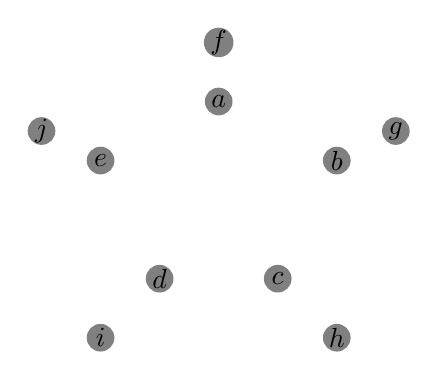
\begin{tikzpicture}[scale=0.75]      
       \foreach \pos/\name in {{(0,2)/a}, {(2,1)/b}, {(-2,1)/e}, {(1,-1)/c}, {(-1,-1)/d}, {(0,3)/f}, {(3,1.5)/g}, {(-3, 1.5)/j}, {(2,-2)/h}, {(-2,-2)/i}} {
           \node[vertex] (\name) at \pos {$\name$};
%           \draw[outline] {\pos circle (4cm)};          
       }


\end{tikzpicture}}
\subfloat[Connection graph]{\label{fig:connec}
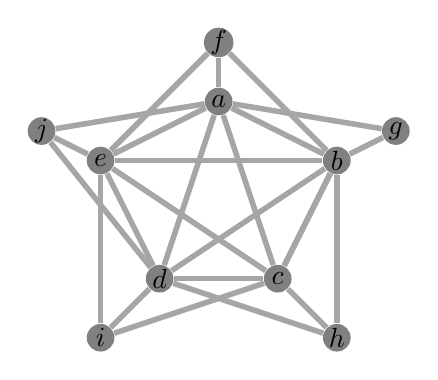
\begin{tikzpicture}[scale=0.75]  
       \foreach \pos/\name in {{(0,2)/a}, {(2,1)/b}, {(-2,1)/e}, {(1,-1)/c}, {(-1,-1)/d}, {(0,3)/f}, {(3,1.5)/g}, {(-3, 1.5)/j}, {(2,-2)/h}, {(-2,-2)/i}} {
           \node[vertex] (\name) at \pos {$\name$};
       }    
       \foreach \source/\sink in {a/f, a/g, a/b, a/c, a/d, a/e, a/j, b/g, b/h, b/c, b/h, b/c, b/d, b/e, b/f, c/h, c/d, c/i, c/e, d/i, d/e, d/h, d/j, e/i, e/f, e/j} {
           \path[real edge] (\source) -- (\sink); 
       }
\end{tikzpicture}}
% Remove empty line
\subfloat[Routing graph]{\label{fig:routing}
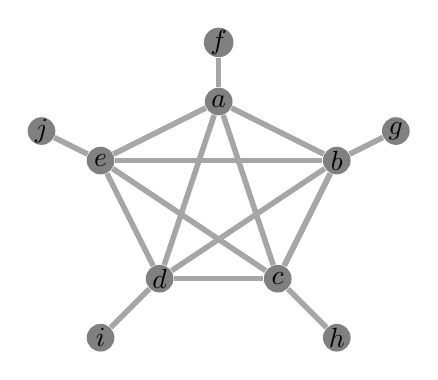
\begin{tikzpicture}[scale=0.75]  
       \foreach \pos/\name in {{(0,2)/a}, {(2,1)/b}, {(-2,1)/e}, {(1,-1)/c}, {(-1,-1)/d}, {(0,3)/f}, {(3,1.5)/g}, {(-3, 1.5)/j}, {(2,-2)/h}, {(-2,-2)/i}} {
           \node[vertex] (\name) at \pos {$\name$};
       }    
       \foreach \source/\sink in {a/f, a/b, a/c, a/d, a/e, b/g, b/c, b/c, b/d, b/e, c/h, c/d, c/e, d/i, d/e, e/j} {
           \path[real edge] (\source) -- (\sink); 
       }
\end{tikzpicture}}
